\documentclass[11pt,a4paper]{article}

\usepackage[a4paper,margin=1in]{geometry}
\usepackage{multicol}
\usepackage{enumitem}
\usepackage{fancyhdr}
\usepackage{setspace}
\usepackage{amsmath}
\usepackage{float}
\usepackage{graphicx}
\usepackage{gvv}
\usepackage{gvv-book}
\usepackage{listings}
\lstset{frame=single, breaklines=true, columns=fullflexible}
\usepackage{caption}
\usepackage[normalem]{ulem}

\pagestyle{fancy}
\fancyhf{}
\fancyhead[L]{GATE 2024}
\fancyhead[C]{\textbf{General Aptitude}}
\fancyfoot[C]{\thepage}

\setlength{\parindent}{0pt}
\setlength{\parskip}{2pt}

\begin{document}

\bibliographystyle{IEEEtran}
\title{GATE 2020 EY - Page 1 Conversion}
\author{EE25BTECH11005- Aditya Mishra}
\maketitle

\rule{\columnwidth}{0.3pt}

\section*{GA - General Aptitude}
\subsection*{Q1 -- Q5 carry one mark each.}

\begin{enumerate}
\item This book, including all its chapters, \rule{1.5cm}{0.15mm} interesting. The students as well as the instructor \rule{1.5cm}{0.15mm} in agreement about it.\hfill {(GATE EY 2020)}
    \begin{enumerate}
    \item is, was
    \item are, are
    \item is, are
    \item were, was
    \end{enumerate}

\item People were prohibited \rule{1.5cm}{0.15mm} their vehicles near the entrance of the main administrative building.\hfill {(GATE EY 2020)}
    \begin{enumerate}
    \item to park
    \item from parking
    \item parking
    \item to have parked
    \end{enumerate}

\item Select the word that fits the analogy:\newline
Do : Undo :: Trust : \rule{1.5cm}{0.15mm}\hfill {(GATE EY 2020)}
    \begin{enumerate}
    \item Entrust
    \item Intrust
    \item Distrust
    \item Untrust
    \end{enumerate}

\item Stock markets \rule{1.5cm}{0.15mm} at the news of the coup.\hfill {(GATE EY 2020)}
    \begin{enumerate}
    \item poised
    \item plunged
    \item plugged
    \item probed
    \end{enumerate}

\item If $P, Q, R, S$ are four individuals, how many teams of size exceeding one can be formed, with $Q$ as a member?\hfill {(GATE EY 2020)}
    \begin{enumerate}
    \item 5
    \item 6
    \item 7
    \item 8
    \end{enumerate}

\subsection*{Q6 -- Q10 carry two marks each.}



    \item Non-performing Assets (NPAs) of a bank in India is defined as an asset, which remains unpaid by a borrower for a certain period of time in terms of interest, principal, or both. Reserve Bank of India (RBI) has changed the definition of NPA thrice during 1993-2004, in terms of the holding period of loans. The holding period was reduced by one quarter each time. In 1993, the holding period was four quarters (360 days).
    Based on the above paragraph, the holding period of loans in 2004 after the third revision was \rule{2cm}{0.15mm} days.\hfill {(GATE EY 2020)}

\begin{enumerate}
    \item 45
    \item 90
    \item 135
    \item 180
\end{enumerate}

\item Select the next element of the series: Z, WV, RQP, \rule{2cm}{0.15mm}\hfill {(GATE EY 2020)}
\begin{enumerate}
    \item LKJI
    \item JIHG
    \item KJIH
    \item NMLK
\end{enumerate}

\item In four-digit integer numbers from 1001 to 9999, the digit group “37” (in the same sequence) appears \rule{2cm}{0.15mm} times.\hfill {(GATE EY 2020)}
\begin{enumerate}
    \item 270
    \item 279
    \item 280
    \item 299
\end{enumerate}


\item Given a semicircle with $O$ as the centre, as shown in the figure, the ratio $\frac{AC+CB}{AB}$ is \rule{2cm}{0.15mm}, where $AC$, $CB$ and $AB$ are chords.\hfill {(GATE EY 2020)}
\begin{center}
\begin{figure}[H]
    \centering
    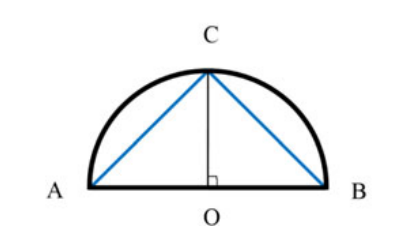
\includegraphics[width=0.8\textwidth]{figs/fig1.png}
    \caption{Semicircle geometry with diameter $AB$, center $O$, and point $C$ on the arc.}
    \label{fig:semicircle-geometry}
\end{figure}
\end{center}
\begin{itemize}
    \item[(A)] $\sqrt{2}$
    \item[(B)] $\sqrt{3}$
    \item[(C)] $2$
    \item[(D)] $3$
\end{itemize}

\item The revenue and expenditure of four different companies P, Q, R and S in 2015 are shown in the figure. If the revenue of company Q in 2015 was 20\% more than that in 2014, and company Q had earned a profit of 10\% on expenditure in 2014, then its expenditure (in million rupees) in 2014 was \rule{2cm}{0.15mm}.\hfill {(GATE EY 2020)}

\begin{center}
\begin{figure}[H]
    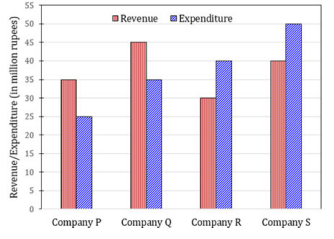
\includegraphics[width=0.8\textwidth]{figs/fig2.png}
\caption{Revenue and Expenditure (in million rupees) of four companies P, Q, R and S in 2015.}
\label{fig:revenue-bar-2015}
\end{figure}
\end{center}
\begin{itemize}
    \item[(A)] 32.7
    \item[(B)] 33.7
    \item[(C)] 34.1
    \item[(D)] 35.1
\end{itemize}
\end{enumerate}

\section*{EY: Ecology and Evolution}

\noindent \textbf{Q1 - Q25 carry one mark each.}
\begin{enumerate}
\item Who among the following was a strong public supporter of Darwin's theory of evolution by natural selection? \hfill {(GATE EY 2020)}

\begin{multicols}{2}
\begin{enumerate}
\item Jean-Baptiste Lamarck
\item Carl Linnaeus
\item Thomas Huxley
\item Gregor Mendel
\end{enumerate}
\end{multicols}

\item Analysis of variance (ANOVA) can be used to compare multiple groups of samples. Select the correct option that reflects the principle behind ANOVA. \hfill {(GATE EY 2020)}

\begin{multicols}{2}
\begin{enumerate}
\item The sum of the squares of the variances is calculated for the groups being compared.
\item The variance ratio is calculated by subtracting each value from the overall mean, squaring the difference, and summing the resulting squared deviations.
\item The variation between groups is compared with the variation within groups.
\item The F value is statistically significant if the mean values between the groups are the same.
\end{enumerate}
\end{multicols}

\item Which of the following information is provided by a phylogenetic tree? \hfill {(GATE EY 2020)}

\begin{multicols}{2}
\begin{enumerate}
\item The topology and the branch lengths of the related taxa.
\item The topology and sequence length of the gene.
\item The sequence length of the gene and tree length.
\item The sequence type and sequence variations within each taxa.
\end{enumerate}
\end{multicols}

\item Myrmecochory refers to seed dispersal by which of the following agents? \hfill {(GATE EY 2020)}

\begin{multicols}{2}
\begin{enumerate}
\item Bats
\item Ants
\item Lizards
\item Birds
\end{enumerate}
\end{multicols}

\item Which of the following is NOT capable of photosynthesis?
\begin{multicols}{2}
\begin{enumerate}
\item Diatoms
\item Phytoplankton
\item Peridophytes
\item Ascomycetes
\end{enumerate}
\end{multicols}

\item Which of the following sensory mechanisms do most frugivorous bats primarily use while foraging?
\begin{multicols}{2}
\begin{enumerate}
\item Olfaction
\item Electromagnetism
\item Vibration
\item Echolocation
\end{enumerate}
\end{multicols}

\item What direct effect does Follicle Stimulating Hormone (FSH) have in vertebrates?
\begin{multicols}{2}
\begin{enumerate}
\item It causes follicles of the duodenum to contract.
\item It causes follicles of the ovaries to grow.
\item It causes follicles of the liver to enlarge.
\item It causes follicles of muscles to contract.
\end{enumerate}
\end{multicols}

\item Juvenile rhesus macaques, who have never seen a leopard before, can learn to show fear response if they see an adult react fearfully to a leopard. What kind of behavioural response is this?
\begin{multicols}{2}
\begin{enumerate}
\item Imprinting
\item Instinct
\item Cultural transmission
\item Mimicry transmission
\end{enumerate}
\end{multicols}

\item In a tropical rainforest during the day, which of the following factors does NOT affect the spectral irradiance at the forest floor?
\begin{multicols}{2}
\begin{enumerate}
\item Angle of the sun on the horizon.
\item Weather conditions of the atmosphere.
\item Structure of the canopy vegetation.
\item Special reflectance of the leaf litter.
\end{enumerate}
\end{multicols}

\item What would an evolutionary biologist hypothesize as the ultimate cause for the presence of colourful dewlaps in lizards?
\begin{multicols}{2}
\begin{enumerate}
\item Colour of dewlaps are formed by pigments in the skin.
\item Colourful dewlaps are formed by folds in the skin.
\item Colourful dewlaps increase mating success.
\item Colourful dewlaps are regions where motor neurons control head movement.
\end{enumerate}
\end{multicols}

\item Which of the following is true about comparisons between herbivorous and carnivorous mammals?
\begin{multicols}{2}
\begin{enumerate}
\item Herbivores have longer digestive tracts and smaller caecum for a given body size than carnivores.
\item Carnivores have longer digestive tracts and smaller caecum for a given body size than herbivores.
\item Herbivores have shorter digestive tracts and smaller caecum for a given body size than carnivores.
\item Carnivores have shorter digestive tracts and smaller caecum for a given body size than herbivores.
\end{enumerate}
\end{multicols}

\item Two isolated populations X and Y have 100 and 10,000 individuals, respectively. Both populations have the same starting allele frequencies of p=0.5 and q=0.5. After 100 generations of genetic drift, which of the following statements is true about the heterozygosity at this locus in these two populations?
\begin{multicols}{2}
\begin{enumerate}
\item The heterozygosity of population X will be more than in population Y.
\item The heterozygosity of population Y will be more than in population X.
\item The heterozygosity of both the populations will be identical.
\item The heterozygosity of these populations will not depend on their population sizes.
\end{enumerate}
\end{multicols}

\item Which of the following criteria is used to define species under the biological species concept?
\begin{multicols}{2}
\begin{enumerate}
\item Niche partitioning
\item Reproductive isolation
\item Morphological divergence
\item Genetic distance
\end{enumerate}
\end{multicols}

\item The abundances of three species (P, Q, and R) were measured along a resource gradient. The resultant pattern is summarized in the figure. Which of the following statements can be inferred from niche theory?\hfill {(GATE EY 2020)}
\begin{center}
\begin{figure}[H]
    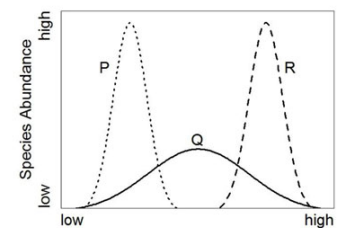
\includegraphics[width=0.8\textwidth]{figs/fig3.png}
\caption{Resource}
\label{fig:q14}
\end{figure}
\end{center}

\begin{multicols}{2}
\begin{enumerate}
\item P is a generalist; Q and R are specialists.
\item Q is a generalist; P and R are specialists.
\item P and Q are generalists; R is a specialist.
\item P and R are generalists; Q is a specialist.
\end{enumerate}
\end{multicols}

\item In the last 3 to 4 decades, the average CO$_2$ concentration in the Earth's atmosphere has increased from $\rule{2cm}{0.15mm}$.
\begin{multicols}{2}
\begin{enumerate}
\item 3 ppm to 4 ppm
\item 30 ppm to 40 ppm
\item 300 ppm to 400 ppm
\item 3000 ppm to 4000 ppm
\end{enumerate}
\end{multicols}

\item What effect does myelination have on neurons?
\begin{multicols}{2}
\begin{enumerate}
\item It increases the transmembrane resistance.
\item It increases the membrane capacitance.
\item It changes the direction of signal propagation.
\item It protects synapses from damage.
\end{enumerate}
\end{multicols}

\item Which of the following processes contributes to an increase in genetic variation?
\begin{multicols}{2}
\begin{enumerate}
\item Genetic drift
\item Directional selection
\item Inbreeding
\item Immigration
\end{enumerate}
\end{multicols}

\item What characteristic do the plant species, sundew (\textit{Drosera capensis}) and Venus fly trap (\textit{Dionaea muscipula}), share?
\begin{multicols}{2}
\begin{enumerate}
\item They are thigmonastic.
\item They are nyctinastic.
\item They are epiphytic.
\item They are endophytic.
\end{enumerate}
\end{multicols}

\item What is the study of fish known as?
\begin{multicols}{2}
\begin{enumerate}
\item Malacology
\item Herpetology
\item Physiology
\item Ichthyology
\end{enumerate}
\end{multicols}

\item On one side of a house, a 50 watt bulb attracts moths at a rate of 30 individuals/minute. On the other side of the house, a 15 watt bulb attracts moths at a rate of 10 individuals/minute. There are 20 bats in the area who are foraging for these moths. According to Ideal Free Distribution, the number of bats near the 15 watt bulb should be \rule{2cm}{0.15mm}.

\item The Simpson’s index of diversity is expressed as:
\[
D = 1 - \sum_{i=1}^n p_i^2
\]
Where $p_i$ is the proportion of the $i$th species, and $n$ is the total number of species.

\begin{center}
\begin{tabular}{ll}
    \textbf{Group I} & \textbf{Group II} \\
    P. Ferrite & 1. Hexagonal Close Packed (HCP) \\
    Q. Austenite & 2. Body Centered Cubic (BCC) \\
    R. Martensite & 3. Body Centered Tetragonal (BCT) \\
    & 4. Face Centered Cubic (FCC)
\end{tabular}
\end{center}

The Simpson’s index of diversity for this dataset is \rule{2cm}{0.15mm}\ (round off to three decimal places).

\item In a botanical garden, tree species P had an average height of 1.5 m, while tree species Q had an average height of 1.8 m. Pooled together, these two tree species had an average height of 1.7 m. From this, one can infer that the number of trees of species Q in the garden was \rule{2cm}{0.15mm} times the number of trees of species P.

\item A fragment of double stranded DNA has 30\% Adenine. The \% GC content in this fragment is \rule{2cm}{0.15mm}.

\item A researcher traps rodents in a small, isolated forest patch. In the first trapping session she captures 24 mice and marks them by notching their ears. In the second trapping session she captures 16 mice, of which 8 are already marked. Assuming that the population is closed (no immigration, emigration, birth, or death), the estimated number of mice in the patch is \rule{2cm}{0.15mm}.\hfill {(GATE EY 2020)}
\item A raptor sitting on a tree sees a rodent on the ground below as shown in the figure (not to scale). If the raptor views the rodent from a height of 10 metres, and the rodent subtends a visual angle of 45$^\circ$ on the raptor's eye, the straight line distance from the raptor to the rodent in metres is \rule{2cm}{0.15mm} (round off to two decimal places). \hfill {(GATE EY 2020)}

\begin{center}
\begin{figure}[H]
    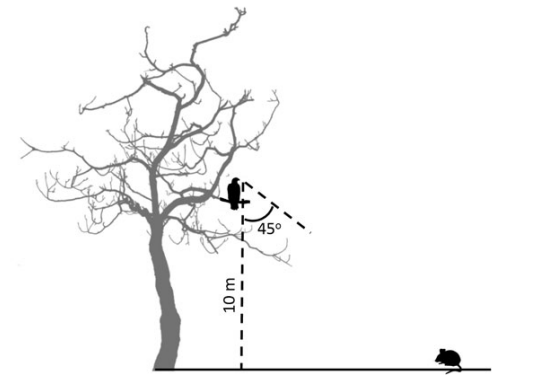
\includegraphics[width=0.8\textwidth]{figs/fig4.png}
\caption{A raptor observes a rodent from a height of 10 meters, subtending a $45^\circ$ angle to the rodent on the ground.}
    \label{fig:raptor-rodent-angle}
\end{figure}
\end{center}
\vspace{1em}

\textbf{Q26 - Q55 carry two marks each.}

\item Beetles of one species have the option of eating plant species X or Y in their environment. Plant species X and Y have the same nutritional quality. When beetle diets comprise a greater proportion of plant X, the population size of beetles increases faster than when beetle diets are dominated by plant Y. Which of the following is NOT a probable explanation for this outcome? \hfill {(GATE EY 2020)}
\begin{multicols}{2}
\begin{enumerate}
\item Xenobiotics in X are physiologically easier for the beetles to detoxify than those in Y.
\item Sequestration of xenobiotics from X by the beetles confers greater protection from bird predators than those from Y.
\item X attracts parasites of the beetles while Y does not.
\item X provides greater protection from bird predators during foraging than does Y.
\end{enumerate}
\end{multicols}

\item A researcher was documenting the number of tree species in a landscape. Within each of three forest types (P, Q, and R), she laid 100 quadrats and documented all the species found in each quadrat. She then plotted the cumulative species richness for these forest types as shown in the figure. Which of the following statements is FALSE? \hfill {(GATE EY 2020)}

\begin{center}
\begin{figure}[H]
    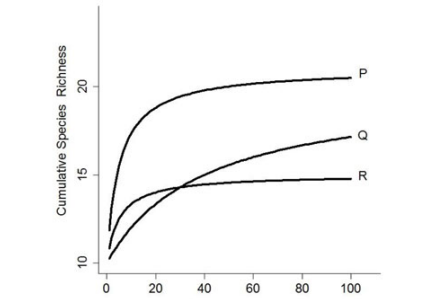
\includegraphics[width=0.8\textwidth]{figs/fig5.png}
\caption{Number of Quadrats}
\label{fig:q26}
\end{figure}
\end{center}

\begin{multicols}{2}
\begin{enumerate}
\item There are more species of trees in P than in R.
\item There are more species of trees in Q than in R.
\item More quadrats are required to estimate species richness in P than in Q.
\item More quadrats are required to estimate species richness in Q than in R.
\end{enumerate}
\end{multicols}
\item Which of the following has an endemic species represented in the Andaman and Nicobar Islands for all taxonomic groups in that column? \hfill {(GATE EY 2020)}

\begin{tabular}{|c|c|c|}
     \hline
     \textbf{Mineral} & \textbf{Modal abundance \brak{\%}} & \textbf{Partition coefficient}\\
     \hline
     Clinopyroxene & $45$ & $0.506$ \\
      \hline
      Orthopyroxene & $40$ & $0.42$ \\
      \hline
      Olivine & $10$ & $0.045$ \\
      \hline
      Plagioclase & $05$ & $0.019$ \\
      \hline
\end{tabular}

\begin{multicols}{2}
\begin{enumerate}
\item Column P
\item Column Q
\item Column R
\item Column S
\end{enumerate}
\end{multicols}

\item The theory of island biogeography predicts that the number of species on islands is determined by: (i) the rate of colonisation, which depends on the distance of the island from the mainland, and (ii) the rate of extinction, which depends on the size of the island. A researcher surveyed two islands with similar habitats and geological history, and found that both islands have the same number of species. Which of the following statement(s) can explain this observation? \hfill {(GATE EY 2020)}

\begin{quote}
P. The islands are of the same size and are at the same distance from the mainland.\\
Q. The islands are of different sizes and are at the same distance from the mainland.\\
R. The islands are of the same size and are at different distances from the mainland.\\
S. The islands are of different sizes and are of different distances from the mainland.
\end{quote}

\begin{multicols}{2}
\begin{enumerate}
\item Only P.
\item Only Q.
\item Both P and S.
\item Both Q and R.
\end{enumerate}
\end{multicols}

\item In marine fauna, Pelagic Larval Duration (PLD) or the amount of time that larvae spend swimming or drifting in the water column affects their dispersal distance. Successful establishment of the larvae on a substrate also depends on finding a suitable habitat after dispersal, which is influenced by whether the habitat is patchy or continuous. Which of the following species will have the lowest population genetic structure ($F_{ST}$) across the same spatial scale? \hfill {(GATE EY 2020)}

\begin{multicols}{2}
\begin{enumerate}
\item Species with high PLD in patchy habitats.
\item Species with high PLD in continuous habitats.
\item Species with low PLD in patchy habitats.
\item Species with low PLD in continuous habitats.
\end{enumerate}
\end{multicols}

\item Every lake in Wakanda has three species of fish: P, Q, and R. Species P is a bottom dweller and substrate feeder, species Q is a mid-column dweller and herbivore, and species R is a surface dweller and piscivore. Which of the following processes best explains this distribution pattern? \hfill {(GATE EY 2020)}
\begin{multicols}{2}
\begin{enumerate}
\item Speciation within one lake followed by dispersal to other lakes.
\item Dispersal between lakes followed by speciation within lakes.
\item Independent speciation events within all the lakes.
\item Speciation within a lake with no dispersal between lakes.
\end{enumerate}
\end{multicols}
\item
Group living can have both benefits (such as protection from predators) and costs (such as competition for resources). The figure depicts net benefit to individuals as a function of group size. Consider a population with more than hundred individuals, where groups do not split, and individuals can choose to either join a group or remain solitary. Given this information, what is the typical group size predicted? \hfill {(GATE EY 2020)}

\begin{center}
\begin{figure}[H]
    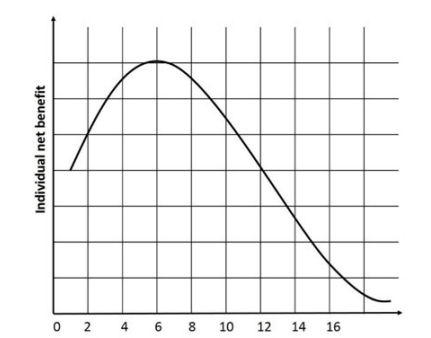
\includegraphics[width=0.8\textwidth]{figs/fig6.png}
\caption{Group Size}
\label{fig:q31}
\end{figure}
\end{center}

\begin{multicols}{2}
\begin{enumerate}
\item Less than 6
\item Equal to 6
\item Between 6 and 12
\item Greater than 12
\end{enumerate}
\end{multicols}

\item
Two species of snails, P and Q, are found in rivers across a range of temperatures that vary from upstream to downstream. An experiment was conducted in which P was removed from a river and the distribution of Q was measured after a few weeks. In another similar river, the reciprocal experiment was conducted in which Q was removed, and the distribution of P was measured after a few weeks. In the graph below, the filled bars plot the distribution of P and Q when both species are present in a river. The open bars plot the distribution of P when Q is removed, and Q when P is removed. Which of the following statements is true? \hfill {(GATE EY 2020)}

\begin{center}
\begin{figure}[H]
    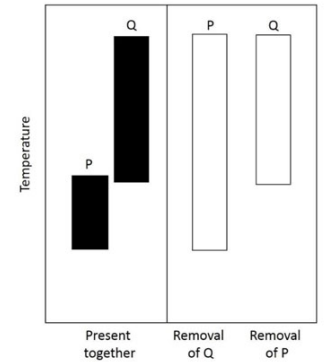
\includegraphics[width=0.8\textwidth]{figs/fig7.png}
\caption{Resource}
\label{fig:q14}
\end{figure}
\end{center}

\begin{multicols}{2}
\begin{enumerate}
\item The realised niche of P is smaller than its fundamental niche.
\item The realised niche of Q is smaller than its fundamental niche.
\item The realised niche is smaller than the fundamental niche for both species.
\item The realised niches of both species are equal.
\end{enumerate}
\end{multicols}
\item
In plants with bisexual flowers (hermaphrodites), mate-choice by females is expected to be important under which of the following cases? \hfill {(GATE EY 2020)}

\begin{quote}
i) Seed set is pollen-limited rather than resource-limited.\\
ii) Obligate self-pollination is present.\\
iii) Seed set is resource-limited rather than pollen-limited.\\
iv) Obligate cross-pollination is present.
\end{quote}

\begin{multicols}{2}
\begin{enumerate}
\item (i) and (ii)
\item (ii) and (iii)
\item (iii) and (iv)
\item (i) and (iv)
\end{enumerate}
\end{multicols}

\item
Match the breeding system of the plants with their pollen:ovule ratio. \hfill {(GATE EY 2020)}
\begin{table}[htbp]
  \centering
  \caption{Table-3}
  \label{table3}
  \begin{tabular}{cc}
  \textbf{Processing Technique} & \textbf{Producct} \\ \\
    P. Calendering & 1. Pipes \\
    Q. Extrusion & 2. Disposable cups \\
    R. Injection moulding & 3. Sheets \\
    S. Thermoforming & 4. Nylon gears \\
  \end{tabular}
\end{table}
\begin{multicols}{2}
\begin{enumerate}
\item P-i, Q-iii, R-ii, S-iv
\item P-ii, Q-i, R-iv, S-iii
\item P-iv, Q-iii, R-i, S-ii
\item P-iii, Q-iv, R-i, S-ii
\end{enumerate}
\end{multicols}

\item
A particular gene sequence from two different species shows molecular clock-like evolution. Which of the following statements is consistent with this observation? \hfill {(GATE EY 2020)}
\begin{multicols}{2}
\begin{enumerate}
\item The two sequences will show a linear decrease in their genetic distance with time.
\item The genetic distance between the two sequences remains constant over time.
\item The rate of evolution for this gene sequence is not constant over time.
\item The two sequences will show a linear increase in their genetic distance with time.
\end{enumerate}
\end{multicols}

\item
An internal parasite of a mammal does not generate its own heat and yet it can maintain a constant body temperature. Which characteristics describe this parasite? \hfill {(GATE EY 2020)}
\begin{multicols}{2}
\begin{enumerate}
\item Homeothermic ectotherm
\item Homeothermic endotherm
\item Poikilothermic ectotherm
\item Poikilothermic endotherm
\end{enumerate}
\end{multicols}

\item
In a population of infinite size, the frequency of two alleles A1 and A2 at a neutral locus are the same. What are the expected genotype frequencies (A1A1, A1A2, A2A2) after 100 generations of random mating? \hfill {(GATE EY 2020)}
\begin{multicols}{2}
\begin{enumerate}
\item 0.25, 0.5, 0.25
\item 0.5, 0.25, 0.25
\item 0.25, 0.25, 0.5
\item 0.05, 0.5, 0.45
\end{enumerate}
\end{multicols}
\item
A certain rodent species shows territoriality, competes for space and food, and their population is at carrying capacity. In the figures, the area within the rectangles (i) to (iv) represents a completely homogenous habitat where resources are distributed throughout, and the grey polygons represent rodent home ranges. Which of the following patterns best represents the expected distribution of home ranges of the rodent species if individuals vary in competitive ability? \hfill {(GATE EY 2020)}

\begin{center}
\begin{figure}[H]
    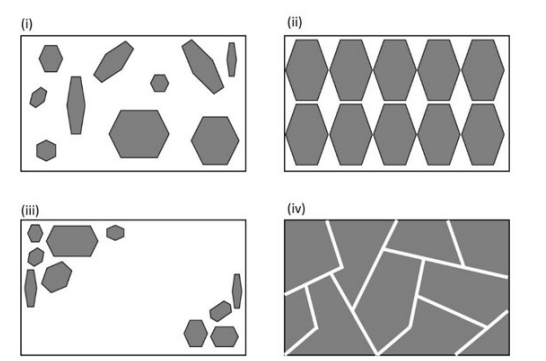
\includegraphics[width=0.8\textwidth]{figs/fig8.png}
\caption{Options}
\label{fig:q14}
\end{figure}
\end{center}
\begin{multicols}{2}
\begin{enumerate}
\item (i)
\item (ii)
\item (iii)
\item (iv)
\end{enumerate}
\end{multicols}

\item
For a given gene there is 5\% DNA sequence divergence between two species, however the protein coded by this gene has identical sequences in the two species. Which of the following types of mutations best explains this pattern in the DNA sequence? \hfill {(GATE EY 2020)}

\begin{multicols}{2}
\begin{enumerate}
\item Nonsense mutation
\item Synonymous substitution
\item Non-synonymous substitution
\item Frame-shift mutation
\end{enumerate}
\end{multicols}

\item
A researcher collects data on plant species composition in two habitats (P and Q) by using 10 quadrats each in both habitats. She calculates the average $\alpha$-diversity and the $\beta$-diversity of each habitat from this data (shown below). Which of the following can be inferred about these habitats? \hfill {(GATE EY 2020)}

\begin{center}
\begin{tabular}{|c|c|c|}
    \hline
    Task & Task time (Seconds) & Immediate predecessor(s) \\
    \hline
    P & 20 & - \\ \hline
    Q & 25 & P \\  \hline
    R & 10 & Q \\ \hline
    S & 15 & Q \\ \hline 
    T & 25 & R, S \\    \hline
\end{tabular}
\end{center}

\begin{multicols}{2}
\begin{enumerate}
\item P and Q have the same total diversity ($\gamma$) and P is more heterogeneous than Q.
\item Q has lower total diversity ($\gamma$) and is more heterogeneous than P.
\item P has greater total diversity ($\gamma$) and is more heterogeneous than Q.
\item Q has greater total diversity ($\gamma$) and is more heterogeneous than P.
\end{enumerate}
\end{multicols}
\item
A certain rodent species shows territoriality, competes for space and food, and their population is at carrying capacity. In the figures, the area within the rectangles (i) to (iv) represents a completely homogenous habitat where resources are distributed throughout, and the grey polygons represent rodent home ranges. Which of the following patterns best represents the expected distribution of home ranges of the rodent species if individuals vary in competitive ability? \hfill {(GATE EY 2020)}

\begin{center}
\begin{figure}[H]
    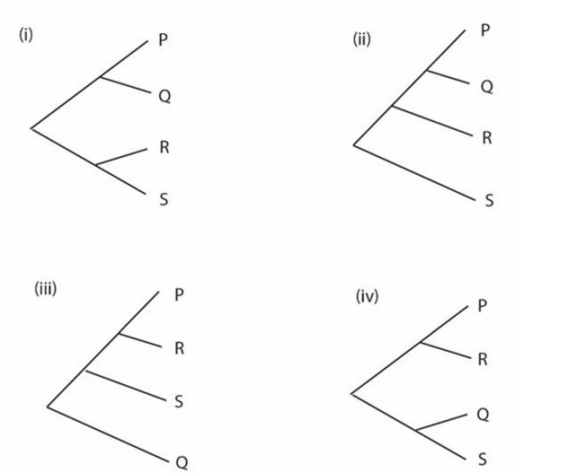
\includegraphics[width=0.8\textwidth]{figs/fig9.png}
\caption{Optionss}
\label{fig:q42}
\end{figure}
\end{center}

\begin{multicols}{2}
\begin{enumerate}
\item (i)
\item (ii)
\item (iii)
\item (iv)
\end{enumerate}
\end{multicols}

\item
For a given gene there is 5\% DNA sequence divergence between two species, however the protein coded by this gene has identical sequences in the two species. Which of the following types of mutations best explains this pattern in the DNA sequence? \hfill {(GATE EY 2020)}

\begin{figure}[H]
\centering
    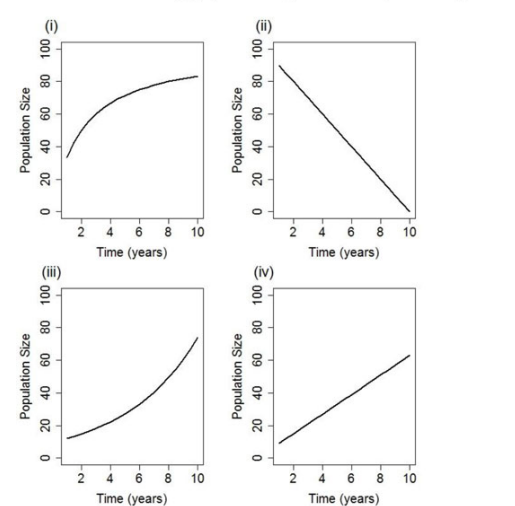
\includegraphics[width=0.8\textwidth]{figs/fig10.png}
\caption{Options}
\label{fig:q43}
\end{figure}

\begin{multicols}{2}
\begin{enumerate}
\item Nonsense mutation
\item Synonymous substitution
\item Non-synonymous substitution
\item Frame-shift mutation
\end{enumerate}
\end{multicols}

\item
In a polyploidization event, tetraploid progeny were formed by diploid parents. Hybridization between the tetraploid and a diploid parent gave rise to sterile triploids. Which of the following best explains why these triploids were sterile? \hfill {(GATE EY 2020)}
\begin{multicols}{2}
\begin{enumerate}
\item Many mutations during polyploidization have no phenotypic effect.
\item Some chromosomes are without homologs during meiosis.
\item Some chromosomes are without homologs during mitosis.
\item All chromosomes have homologs during mitosis.
\end{enumerate}
\end{multicols}

\item
Blood tests are often used to screen for potential diseases. For a particular disease:\\
(i) Of 1000 persons who tested negative ($T'$), 1 person had the disease ($D$); $Pr(D|T').$\\
(ii) Of 10 persons who tested positive ($T$), 1 person had the disease ($D$); $Pr(D|T)$.\\
From this we can calculate\\\newline
$\displaystyle \frac{Pr(D|T)}{Pr(D|T')} = \frac{1/10}{1/1000} = 100$\\
What can be inferred from this value? \hfill {(GATE EY 2020)}
\begin{multicols}{2}
\begin{enumerate}
\item 100 people have the disease but they will not test positive.
\item 1 in 100 people have the disease and they will test positive.
\item 100 in 1000 people have the disease and their blood tests will be inconclusive.
\item People with positive tests are 100 times more likely to have the disease than people with negative tests.
\end{enumerate}
\end{multicols}

\item
The relative frequency distributions of values of a trait in two samples, P and Q, are shown in the figure. Which of the following statements is consistent with the figure? \hfill {(GATE EY 2020)}


\begin{figure}[H]
\centering
    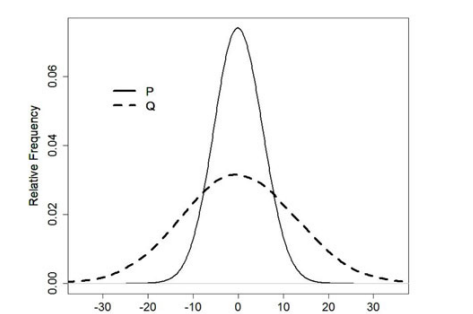
\includegraphics[width=0.8\textwidth]{figs/fig11.png}
\caption{Trait value}
\label{fig:q46}
\end{figure}


\begin{multicols}{2}
\begin{enumerate}
\item P has a higher mean than Q; Q has a higher variance than P.
\item P has a higher mean than Q; P has a higher variance than Q.
\item P and Q have the same mean; Q has a higher variance than P.
\item P and Q have the same mean; P has a higher variance than Q.
\end{enumerate}
\end{multicols}
\item
In a polyploidization event, tetraploid progeny were formed by diploid parents. Hybridization between the tetraploid and a diploid parent gave rise to sterile triploids. Which of the following best explains why these triploids were sterile? \hfill {(GATE EY 2020)}
\begin{multicols}{2}
\begin{enumerate}
\item Many mutations during polyploidization have no phenotypic effect.
\item Some chromosomes are without homologs during meiosis.
\item Some chromosomes are without homologs during mitosis.
\item All chromosomes have homologs during mitosis.
\end{enumerate}
\end{multicols}

\item Consider the function $f(x) = \left| \frac{e^{\beta x}}{\beta} \right|$ \\
Which of the following graphs represents the relationship between $x$ and $f(x)$?

\begin{figure}[H]
\centering
    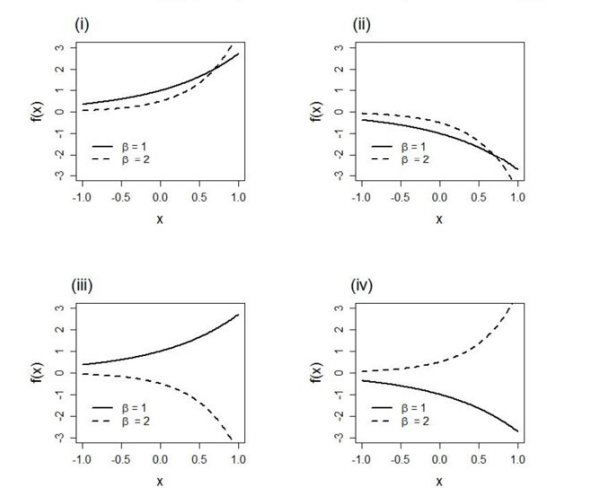
\includegraphics[width=0.8\textwidth]{figs/fig12.png}
\caption{Options}
\label{fig:q48}
\end{figure}

\item
The relative frequency distributions of values of a trait in two samples, P and Q, are shown in the figure. Which of the following statements is consistent with the figure? \hfill {(GATE EY 2020)}


\begin{figure}[H]
\centering
    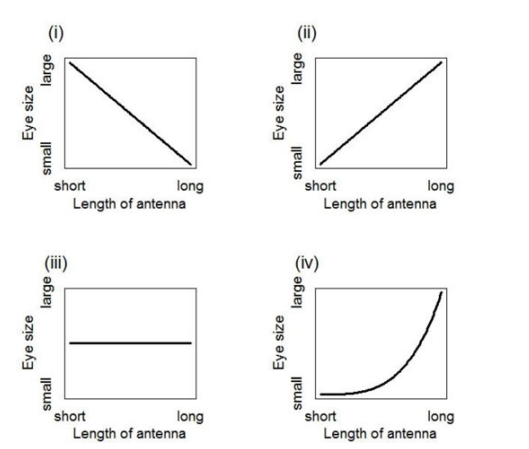
\includegraphics[width=0.8\textwidth]{figs/fig13.png}
\caption{Options}
\label{fig:q49}
\end{figure}


\begin{multicols}{2}
\begin{enumerate}
\item P has a higher mean than Q; Q has a higher variance than P.
\item P has a higher mean than Q; P has a higher variance than Q.
\item P and Q have the same mean; Q has a higher variance than P.
\item P and Q have the same mean; P has a higher variance than Q.
\end{enumerate}
\end{multicols}
\item
A researcher compared grass species richness in a 10 m $\times$ 10 m plot immediately before (T$_0$) and 100 days after (T$_{100}$) a fire. She observed that species richness was higher at T$_{100}$ than at T$_0$. Which of the following data is required for her to conclude that species richness increased because of the fire? \hfill {(GATE EY 2020)}
\begin{multicols}{2}
\begin{enumerate}
\item Grass species richness of a 10 m $\times$ 10 m plot in a nearby area that also burned.
\item Grass species richness of a 10 m $\times$ 10 m plot only at T$_{100}$ in a nearby area that did not burn.
\item Grass species richness of a 10 m $\times$ 10 m plot at both T$_0$ and T$_{100}$ in a nearby area that did not burn.
\item Grass species richness of the same 10 m $\times$ 10 m plot every 10 days after the fire until T$_{100}$.
\end{enumerate}
\end{multicols}

\item
Following a gene duplication event, the duplicated copy often loses function and is called a pseudogene. In the absence of positive selection, which of the following is true about these genes? \hfill {(GATE EY 2020)}
\begin{multicols}{2}
\begin{enumerate}
\item The functional gene will accumulate mutations more rapidly than the pseudogene.
\item The pseudogene will accumulate mutations more rapidly than the functional gene.
\item Both the functional gene and the pseudogene will accumulate mutations at the same rate.
\item The pseudogene will not accumulate mutations.
\end{enumerate}
\end{multicols}

\item
Which of the figures represents the expected relationship between parental care and the number of offspring produced across taxa? \hfill {(GATE EY 2020)}

\begin{figure}[H]
\centering
    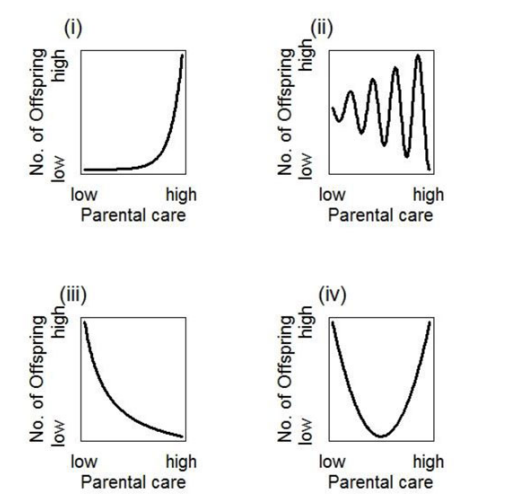
\includegraphics[width=0.8\textwidth]{figs/fig14.png}
\caption{Options}
\label{fig:q48}
\end{figure}

\begin{multicols}{2}
\begin{enumerate}
\item (i)
\item (ii)
\item (iii)
\item (iv)
\end{enumerate}
\end{multicols}
\item
Match the following plant traits with the correct plant group/family: \hfill {(GATE EY 2020)}
\begin{table}[h!]
\centering
\begin{tabular}{|c|c|c|c|}
\hline
\textbf{Pressure} & \textbf{Temperature} & \multicolumn{2}{c|}{\textbf{Specific enthalpy}} \\ \cline{3-4} 
\textbf{(kPa)} & \textbf{($^\circ$C)} & $h_f$ (kJ/kg) & $h_g$ (kJ/kg) \\ \hline
150.9 & $-20$ & 17.82 & 178.74 \\ \hline
500 & 15.6 & 50.64 & 195.01 \\ \hline
\end{tabular}
\end{table}

\begin{multicols}{2}
\begin{enumerate}
\item P-iv, Q-v, R-i, S-ii
\item P-ii, Q-iv, R-iii, S-i
\item P-i, Q-ii, R-iii, S-iv
\item P-iii, Q-v, R-i, S-ii
\end{enumerate}
\end{multicols}

\item
In a population of 100 individuals of a diploid organism with 1:1 sex ratio, the probability of fixation of a new neutral mutation is \rule{2cm}{0.15mm} (round off to three decimal places). \hfill {(GATE EY 2020)}

\item
The binomial probability of obtaining exactly $k$ successes in $n$ trials, where the probability of success in a single trial is $p$, is given by:\\
\[
Pr(x=k) =  {}^nC_k{} \cdot (p)^k \cdot (1-p)^{n-k}
\]
Here, $^nC_k$ notation refers to number of combinations for $k$ successes among $n$ trials. With a fair and unbiased coin, the probability of getting 2 HEADS in a trial with 5 tosses is \rule{2cm}{0.15mm} (round off to two decimal places). \hfill {(GATE EY 2020)}

\item
A petrified wood fossil was discovered with 8 g of $^{14}$C. The decay of $^{14}$C over time is given by:\\
\[
N_T = N_0 \, e^{-0.0001216T}
\]
If the half-life of $^{14}$C is 5700 years, and the fossil initially had 32 g of $^{14}$C, the age of the fossil in years is \rule{2cm}{0.15mm}. \hfill {(GATE EY 2020)}
\newpage
\subsection{Answer Key EY: Ecology and Evolution}
\begin{table}[htbp]
  \centering
  \caption{Table-6}
  \label{tab:tables/table6.tex}
  \begin{tabular}{cc}
  \textbf{Reagent} & \textbf{Function} \\ \\
    P.Ammonia  & 1. Prevent storage hardening \\
    Q. Hydroxylamine & 2. Delay plugging mechanism \\
    R. Formic acid & 3. Stabilizer \\
    S. Ethephone & 4. Coagulating agent \\
  \end{tabular}
\end{table}
\end{enumerate}



\end{document}